\documentclass[tikz,border=2pt]{standalone}
\usepackage{libertine}
\usepackage{pgfplots}
\pgfplotsset{compat=1.18}

\definecolor{nativeblue}{HTML}{4C78A8}
\definecolor{tailorange}{HTML}{F58518}
\definecolor{gapred}{HTML}{E45756}
\definecolor{exactgreen}{HTML}{54A24B}

\begin{document}
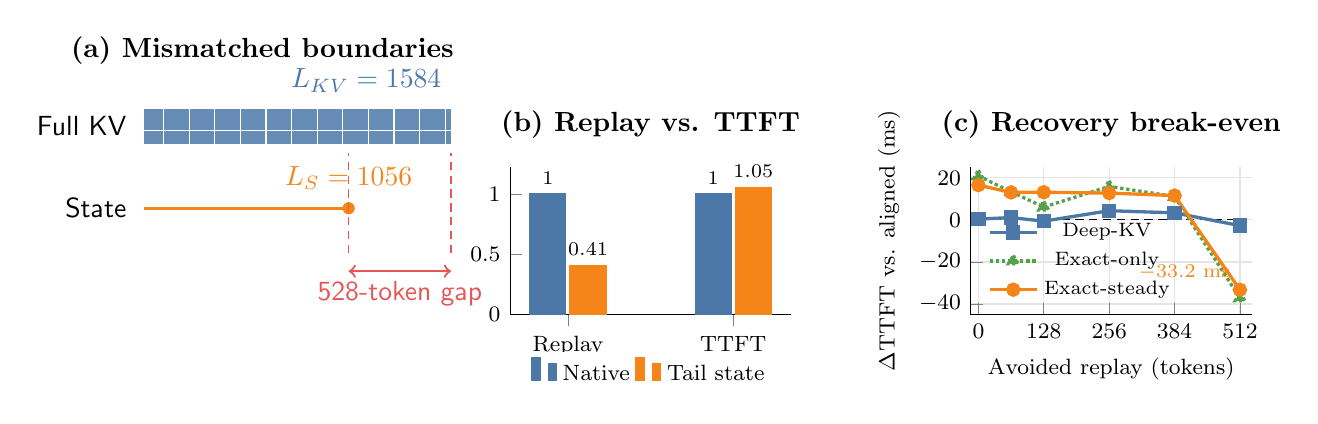
\begin{tikzpicture}[font=\sffamily]
  % (a) Heterogeneous recovery boundaries.
  \begin{scope}
    \node[anchor=west,font=\bfseries] at (0,3.65)
      {(a) Mismatched boundaries};
    \node[anchor=east] at (0.95,2.70) {Full KV};
    \node[anchor=east] at (0.95,1.65) {State};

    \fill[nativeblue!85] (1.05,2.47) rectangle (4.95,2.91);
    \draw[white,thin] (1.05,2.47) grid[xstep=0.325,ystep=0.44] (4.95,2.91);
    \draw[tailorange,very thick] (1.05,1.65) -- (3.65,1.65);
    \fill[tailorange] (3.65,1.65) circle (2.2pt);

    \draw[gapred,<->,thick] (3.65,0.85) -- (4.95,0.85)
      node[midway,below] {528-token gap};
    \draw[densely dashed,gapred] (3.65,1.08) -- (3.65,2.35);
    \draw[densely dashed,gapred] (4.95,1.08) -- (4.95,2.35);

    \node[anchor=south,tailorange] at (3.65,1.76) {$L_S=1056$};
    \node[anchor=south east,nativeblue] at (4.95,3.00) {$L_{KV}=1584$};
  \end{scope}

  % (b) Less replay does not imply lower TTFT.
  \begin{axis}[
    at={(5.70cm,0.30cm)}, anchor=south west,
    width=5.15cm, height=3.45cm,
    title={(b) Replay vs. TTFT},
    title style={font=\bfseries,yshift=1pt},
    ybar=1.5pt, bar width=13pt,
    symbolic x coords={Replay,TTFT}, xtick=data,
    ymin=0, ymax=1.22,
    ytick={0,0.5,1.0},
    axis x line*=bottom, axis y line*=left,
    enlarge x limits=0.35,
    legend style={draw=none,at={(0.5,-0.25)},anchor=north,
                  legend columns=2,font=\footnotesize},
    tick label style={font=\footnotesize},
    label style={font=\footnotesize},
    nodes near coords,
    every node near coord/.append style={font=\scriptsize,anchor=south},
  ]
    \addplot[fill=nativeblue,draw=nativeblue]
      coordinates {(Replay,1.000) (TTFT,1.000)};
    \addplot[fill=tailorange,draw=tailorange]
      coordinates {(Replay,0.407) (TTFT,1.053)};
    \legend{Native,Tail state}
  \end{axis}

  % (c) Exact recovery has a request-dependent break-even.
  \begin{axis}[
    at={(11.55cm,0.30cm)}, anchor=south west,
    width=5.15cm, height=3.45cm,
    title={(c) Recovery break-even},
    title style={font=\bfseries,yshift=1pt},
    xlabel={Avoided replay (tokens)},
    ylabel={$\Delta$TTFT vs. aligned (ms)},
    xmin=-15, xmax=535, ymin=-45, ymax=25,
    xtick={0,128,256,384,512}, ytick={-40,-20,0,20},
    axis x line*=bottom, axis y line*=left,
    tick label style={font=\footnotesize},
    label style={font=\footnotesize},
    grid=major, grid style={gray!20},
    legend style={draw=none,fill=none,font=\scriptsize,
                  at={(0.03,0.03)},anchor=south west},
  ]
    \addplot[black,densely dashed,thin,forget plot]
      coordinates {(0,0) (512,0)};
    \addplot[nativeblue,very thick,mark=square*,mark options={fill=nativeblue}]
      coordinates {(0,0.40) (64,1.13) (128,-0.58) (256,4.39)
                   (384,3.37) (512,-2.72)};
    \addplot[exactgreen,very thick,densely dotted,mark=triangle*,
             mark options={fill=exactgreen}]
      coordinates {(0,20.98) (64,13.40) (128,6.12) (256,15.95)
                   (384,11.14) (512,-37.14)};
    \addplot[tailorange,very thick,mark=*,mark options={fill=tailorange}]
      coordinates {(0,16.56) (64,13.09) (128,13.17) (256,12.78)
                   (384,11.59) (512,-33.22)};
    \legend{Deep-KV,Exact-only,Exact-steady}
    \node[font=\scriptsize,anchor=south east,tailorange]
      at (axis cs:512,-33.22) {$-33.2$ ms};
  \end{axis}
\end{tikzpicture}
\end{document}
